\documentclass[11pt,letterpaper]{article}

% ---------------------------------------------------------------------
% Paquetes
% ---------------------------------------------------------------------
\usepackage[utf8]{inputenc}
\usepackage[T1]{fontenc}
\usepackage[spanish]{babel}
\usepackage[margin=1in]{geometry}
\usepackage{graphicx}
\usepackage{float} % [H]: ancla tablas/figuras exactamente donde se escriben, sin drift
\usepackage{listings}
\usepackage{xcolor}
\usepackage{booktabs}
\usepackage{longtable}
\usepackage{amsmath}
\usepackage{hyperref}
\usepackage{enumitem}
\usepackage{fancyhdr}
\usepackage{titlesec}
\usepackage{caption}
\usepackage{tikz}
\usetikzlibrary{shapes.geometric,arrows.meta,positioning,calc,fit}

% Estilos TikZ compartidos por los diagramas de flujo
\tikzset{
    blk/.style={rectangle, draw, rounded corners=2pt, align=center,
                minimum height=0.8cm, text width=3.6cm, font=\small, fill=blue!6},
    io/.style={rectangle, draw, rounded corners=8pt, align=center,
               minimum height=0.8cm, text width=3.6cm, font=\small, fill=green!10},
    dec/.style={diamond, draw, aspect=2.2, align=center, inner sep=1pt,
                font=\scriptsize, fill=yellow!15},
    key/.style={rectangle, draw, rounded corners=2pt, align=center,
                minimum height=0.8cm, text width=3.9cm, font=\small, fill=orange!12},
    arr/.style={-{Stealth[length=2.5mm]}, thick},
    msg/.style={-{Stealth[length=2.5mm]}, thick, color=red!70!black},
    lbl/.style={font=\scriptsize, midway, fill=white, inner sep=1pt},
}

\hypersetup{
    colorlinks=true,
    linkcolor=black,
    citecolor=black,
    urlcolor=blue,
    pdftitle={Proyecto 2 - Bruteforce DES con Open MPI},
}

\lstset{
    basicstyle=\ttfamily\small,
    breaklines=true,
    frame=single,
    backgroundcolor=\color{gray!10},
    columns=fullflexible,
    keepspaces=true,
    showstringspaces=false,
}

\pagestyle{fancy}
\fancyhf{}
\fancyhead[L]{Computación Paralela y Distribuida}
\fancyhead[R]{Proyecto 2 — Bruteforce DES}
\fancyfoot[C]{\thepage}

\titleformat{\section}{\normalfont\Large\bfseries}{\thesection}{1em}{}
\titleformat{\subsection}{\normalfont\large\bfseries}{\thesubsection}{1em}{}

\setlength{\parskip}{0.5em}
\setlength{\parindent}{0pt}

\begin{document}

% =======================================================================
% CARÁTULA
% =======================================================================
\begin{titlepage}
    \centering
    \vspace*{1cm}

    {\Large \textbf{Universidad del Valle de Guatemala}}\\[0.3cm]
    {\large Facultad de Ingeniería}\\[0.3cm]
    {\large Computación Paralela y Distribuida}\\[2cm]

    \rule{\linewidth}{0.5mm} \\[0.4cm]
    {\huge \textbf{Proyecto 2}}\\[0.2cm]
    {\LARGE Búsqueda por fuerza bruta de llaves DES\\ con Open MPI y OpenMP}\\[0.4cm]
    \rule{\linewidth}{0.5mm} \\[2cm]

    \begin{flushleft}
        \textbf{Docente}\\
        \quad Ing. Juan Luis García\\[0.3cm]
        \textbf{Integrantes}\\
        \quad -- José Mérida\\
        \quad -- Javier España\\
        \quad -- Angel Esquit\\[0.5cm]
        \textbf{Repositorio}\\
        \quad \url{https://github.com/angelesquit/pry2-cpd}\\
    \end{flushleft}

    \vfill

    {\large Semestre 2, 2026}\\
    {\large Guatemala}

\end{titlepage}

\tableofcontents
\newpage

% =======================================================================
\section{Introducción}
% =======================================================================

El cifrado DES (\textit{Data Encryption Standard}) fue el estándar de
cifrado simétrico de bloque dominante desde su adopción por el NIST en
1977 hasta finales de la década de 1990 (NIST, 1999).\footnote{FIPS PUB 46-3, \url{https://csrc.nist.gov/publications/detail/fips/46/3/final}.} Fue formalmente
reemplazado por AES porque su espacio de llaves de 56 bits efectivos
se volvió computacionalmente inseguro frente al poder de cómputo
disponible (Stallings, 2017, cap. 3). Esa debilidad es precisamente lo
que hace de DES un caso de estudio clásico para la computación
paralela. Su espacio de búsqueda de $2^{56}$ llaves es demasiado
grande para ejecución manual, pero abarcable con cómputo paralelo
moderno. Un ataque de fuerza bruta que resulta impráctico en una sola
máquina puede volverse tratable repartiendo el espacio de llaves entre
múltiples procesos y, eventualmente, múltiples máquinas.

Este proyecto implementa y analiza dicho ataque de fuerza bruta sobre
DES. Parte de una versión secuencial de referencia y evoluciona hacia
distintas estrategias de paralelización con \textbf{Open MPI}, una
versión \textit{naive} que particiona el espacio de llaves en bloques
contiguos iguales, y tres acercamientos alternativos pensados para
corregir las limitaciones observadas en la versión naive
(\textit{master-worker} dinámico, recorrido intercalado o
\textit{striding}, y partición con \textit{shuffle} pseudo-aleatorio).
Además se implementó una versión híbrida que combina paso de mensajes
(MPI, memoria distribuida) con memoria compartida (\textbf{OpenMP})
dentro de cada proceso. Esto aprovecha los núcleos disponibles en cada
nodo sin necesidad de lanzar un proceso MPI por núcleo.

El análisis estudia cómo cambia el tiempo según la
posición de la llave, qué speedup y eficiencia se obtienen y qué
costos tiene cada estrategia. Las Partes A y B siguen la estructura de
la rúbrica y el documento cierra con conclusiones, anexos y bibliografía.

% =======================================================================
\section{Parte A --- Antecedentes}
% =======================================================================

\subsection{Investigación sobre DES}

DES opera sobre bloques de 64 bits de texto plano utilizando una llave
de 64 bits (56 bits efectivos más 8 bits de paridad, uno por cada
byte). El algoritmo se estructura en las siguientes etapas. Están
descritas en el estándar oficial FIPS PUB 46-3 (NIST, 1999) y
resumidas por Stallings (2017, cap. 3).

\begin{enumerate}
    \item \textbf{Permutación inicial (IP).} reordena los 64 bits del
    bloque de entrada según una tabla fija, sin aportar seguridad
    criptográfica directa pero facilitando la carga en hardware de la
    época.
    \item \textbf{16 rondas de Feistel.} en cada ronda, el bloque se
    divide en una mitad izquierda $L$ y una mitad derecha $R$ de 32
    bits cada una. La función de ronda $F$ se aplica sobre $R$ junto
    con la subllave de esa ronda, y el resultado se combina mediante
    XOR con $L$. Al finalizar la ronda, $L$ y $R$ se intercambian.
    \item \textbf{Función $F$.} expande $R$ de 32 a 48 bits mediante la
    tabla de expansión $E$, realiza XOR con la subllave de 48 bits de la
    ronda, pasa el resultado por 8 \textit{S-boxes} (sustitución no
    lineal, cada una mapea 6 bits de entrada a 4 bits de salida) y
    aplica una permutación final $P$.
    \item \textbf{Generación de subllaves (\textit{key schedule}).} la
    llave original de 64 bits pasa por la permutación PC-1 (que
    descarta los 8 bits de paridad, dejando 56 bits efectivos),
    rotaciones de bits por ronda, y la permutación PC-2, generando las
    16 subllaves de 48 bits usadas en cada ronda.
    \item \textbf{Permutación final ($IP^{-1}$).} inversa de la
    permutación inicial, produce el bloque de texto cifrado de 64 bits.
\end{enumerate}

El descifrado reutiliza exactamente el mismo algoritmo, aplicando las
16 subllaves en orden inverso. Esta simetría es la razón por la que, en
este proyecto, \texttt{des\_decrypt} y \texttt{des\_encrypt}
(Sección~\ref{sec:anexo1}) comparten casi todo su código.

La vulnerabilidad estructural de DES frente a fuerza bruta no proviene
de un defecto en las S-boxes ni en el esquema de Feistel en sí. Ambos
se han mantenido razonablemente resistentes a criptoanálisis
diferencial y lineal. El problema real es el tamaño de su espacio de
llaves efectivo, $2^{56} \approx 7.2 \times 10^{16}$ combinaciones. Ese
número era impracticable de recorrer secuencialmente en el hardware de
los años 70. Sin embargo, el proyecto EFF DES Cracker demostró en 1998
que una máquina dedicada podía romper DES en menos de 3 días. Hoy en
día, hardware de propósito general con suficiente paralelismo puede
reducir ese tiempo drásticamente.

\clearpage
\subsection{Diagrama de flujo del algoritmo DES}
\label{sec:flujo-des}

La Figura~\ref{fig:des-flujo} muestra el cifrado de un bloque de 64 bits
(columna izquierda), la generación de subllaves (columna derecha) y el
detalle de la función de ronda $F$ (parte inferior). Para descifrar se
usa exactamente el mismo diagrama aplicando las subllaves en el orden
$K_{16}, K_{15}, \ldots, K_1$.

\begin{figure}[H]
\centering
\begin{tikzpicture}[node distance=0.55cm]
  % --- Columna de datos
  \node[io] (pt) {Texto plano\\(64 bits)};
  \node[blk, below=of pt] (ip) {Permutaci\'on inicial $IP$};
  \node[blk, below=of ip] (split) {Divisi\'on del bloque\\$L_0$ (32 b) $\mid$ $R_0$ (32 b)};
  \node[blk, below=of split, fill=blue!14, text width=4.6cm] (round)
       {\textbf{Ronda $i = 1,\ldots,16$}\\
        $L_i = R_{i-1}$\\
        $R_i = L_{i-1} \oplus F(R_{i-1}, K_i)$};
  \node[blk, below=of round] (swap) {Intercambio final\\$(R_{16}\,\Vert\,L_{16})$};
  \node[blk, below=of swap] (ipinv) {Permutaci\'on final $IP^{-1}$};
  \node[io, below=of ipinv] (ct) {Texto cifrado\\(64 bits)};
  \foreach \a/\b in {pt/ip, ip/split, split/round, round/swap, swap/ipinv, ipinv/ct}
      \draw[arr] (\a) -- (\b);
  % bucle de rondas
  \draw[arr] (round.east) -- ++(0.55,0) |- node[lbl, pos=0.25, right]{$i<16$} (round.north east |- split.south east) ;

  % --- Columna de subllaves
  \node[io, right=3.6cm of pt] (k64) {Llave (64 bits)\\56 \'utiles + 8 paridad};
  \node[key, below=of k64] (pc1) {$PC\text{-}1$ (descarta paridad)\\$\to$ 56 bits};
  \node[key, below=of pc1] (cd) {Divisi\'on $C_0$ (28 b) $\mid$ $D_0$ (28 b)};
  \node[key, below=of cd] (rot) {Rotaci\'on circular a la izquierda\\de $C_i$, $D_i$ (1 o 2 posiciones)};
  \node[key, below=of rot] (pc2) {$PC\text{-}2$ (selecci\'on)\\$\to$ subllave $K_i$ (48 bits)};
  \foreach \a/\b in {k64/pc1, pc1/cd, cd/rot, rot/pc2}
      \draw[arr] (\a) -- (\b);
  \draw[arr] (pc2.west) -- node[lbl, above]{$K_i$} (round.east |- pc2.west) -- (round.east);
  \draw[arr] (rot.east) -- ++(0.5,0) |- node[lbl, pos=0.25, right]{$\times 16$} (cd.east);

  % --- Funcion F
  \node[io, below=1.4cm of ct, xshift=-4.2cm, text width=2.6cm] (fin) {$R_{i-1}$ (32 bits)};
  \node[key, right=0.5cm of fin, text width=2.4cm] (e) {Expansi\'on $E$\\32 $\to$ 48 bits};
  \node[key, right=0.5cm of e, text width=2.0cm] (x) {XOR con $K_i$\\(48 bits)};
  \node[key, right=0.5cm of x, text width=2.4cm] (sb) {8 S-boxes\\6 $\to$ 4 bits c/u};
  \node[key, right=0.5cm of sb, text width=2.0cm] (p) {Permutaci\'on $P$\\(32 bits)};
  \foreach \a/\b in {fin/e, e/x, x/sb, sb/p}
      \draw[arr] (\a) -- (\b);
  \node[font=\small\bfseries, above=0.5cm of x] (ftitle) {Funci\'on $F(R_{i-1}, K_i)$};
  \node[draw, dashed, fit=(fin)(e)(x)(sb)(p)(ftitle), inner sep=6pt] {};
\end{tikzpicture}
\caption{Diagrama de flujo de DES con el cifrado de un bloque, generaci\'on de
subllaves y funci\'on de ronda $F$.}
\label{fig:des-flujo}
\end{figure}
\clearpage

\subsection{Resultados de la versión secuencial}
\label{sec:secuencial}

La versión secuencial (\texttt{src/bruteforce/secuencial.c}) recorre
linealmente el rango $[0, \texttt{max\_key}]$ probando cada llave con
\texttt{try\_key}, y sirve como línea base para calcular el speedup de
todas las versiones paralelas.

\begin{table}[H]
\centering
\small
\begin{tabular}{lrrr}
\toprule
\textbf{Llave buscada} & \textbf{Iteraciones} & \textbf{Tiempo (s)} & \textbf{Tasa (llaves/s)} \\
\midrule
123{,}456 (base, Parte B.2)               & 123{,}457    & 0.039  & $3.17\times10^{6}$ \\
67{,}108{,}865 ($N/2+1$, fácil)          & 67{,}108{,}866 & 20.890 & $3.21\times10^{6}$ \\
83{,}886{,}080 ($N/2+N/8$, media)        & 83{,}886{,}081 & 26.097 & $3.21\times10^{6}$ \\
29{,}498{,}402 ($N/7+N/13+1$, difícil)   & 29{,}498{,}403 & 9.197  & $3.21\times10^{6}$ \\
\bottomrule
\end{tabular}
\caption{Versión secuencial, $N=2^{27}$ (\texttt{scripts/benchmark.sh},
\texttt{resultados\_benchmark.csv}). La secuencial prueba las llaves en
orden y se detiene al encontrar la correcta, así que hace
exactamente \textit{llave}$+1$ iteraciones, y su tiempo es
\textit{iteraciones}$/$\textit{tasa} con una tasa constante de
$\approx3.21\times10^{6}$ llaves/s. Por eso la tabla es lineal y sirve
como línea base ($T_{seq}$) y para medir la tasa, no como análisis.
Los nombres fácil/media/difícil describen qué tan favorable es la llave
para naive con 4 procesos (Sección~\ref{sec:comparativa}), no para la
secuencial, para la cual la llave más grande es la más lenta.}
\label{tab:secuencial}
\end{table}

El espacio de llaves real de DES, $N = 2^{56}$, es intratable en la
práctica para esta comparación. A la tasa de verificación medida en
esta máquina ($\approx 3.2 \times 10^{6}$ llaves/segundo por núcleo),
recorrer $2^{56}$ llaves secuencialmente tomaría aproximadamente
$2.25 \times 10^{9}$ segundos, unos 71 años. Por eso se sustituyó
$N=2^{56}$ por un espacio efectivo reducido
$N_{\text{ef}} = 2^{27} \approx 1.34 \times 10^{8}$ para los casos
fácil/media/difícil de la Parte B.5, siguiendo la misma lógica de
fracciones que propone el enunciado. Esto preserva el fenómeno que se
quiere observar, la posición relativa dentro del segmento, con tiempos
de ejecución de segundos en lugar de décadas.

\subsection{Evidencia de correcto funcionamiento del wrapper DES}
\label{sec:des-wrapper}

Se verificó el correcto funcionamiento del wrapper de cifrado/descifrado
ejecutando el ciclo completo de cifrar y luego descifrar con la misma
llave, confirmando que se recupera exactamente el texto original.

\begin{lstlisting}[language=bash]
bin/cifrar data/texto.txt data/texto_cifrado.bin 42
bin/descifrar data/texto_cifrado.bin 42
# Salida esperada: "Esta es una prueba de proyecto 2"
\end{lstlisting}

Ver Figura~\ref{fig:b1} (Sección~\ref{sec:b1}).

Las funciones \texttt{des\_encrypt} y \texttt{des\_decrypt} de
\texttt{src/common/des.c} son un wrapper sobre la API de DES de
OpenSSL (\texttt{DES\_ecb\_encrypt}, OpenSSL Project, 2024).\footnote{\url{https://www.openssl.org/docs/man3.0/man3/DES_ecb_encrypt.html}.} Se usa en
lugar de la cabecera histórica \texttt{rpc/des\_crypt.h}, que ya no
está disponible en distribuciones modernas de Linux. La llave,
representada como un entero \texttt{long}, se empaqueta en un bloque
de 8 bytes a razón de 7 bits útiles por byte, con el bit 0 siempre en
0, antes de construir el \textit{key schedule} con
\texttt{DES\_set\_key\_unchecked}. Esta función, a diferencia de
\texttt{DES\_set\_key}, no valida ni fuerza los bits de paridad.

Se empaquetan sólo 7 bits por byte porque DES ignora el bit menos
significativo de cada byte (paridad), así que con los 8 bits crudos llaves que
difieren sólo en esos bits darían el mismo \textit{key schedule}. Así
cada valor de \texttt{long} en $[0, 2^{56}-1]$ corresponde a una llave
DES distinta, y el espacio efectivo recorrido es de $2^{56}$ llaves
distinguibles, como indica el enunciado.

\subsection{Explicación de rutinas clave}

Las siguientes rutinas de \texttt{src/common/} son compartidas por los
8 binarios del proyecto (cifrado, descifrado y las 6 versiones de
bruteforce). Su detalle de entradas/salidas se amplía en el Anexo 1
(Sección~\ref{sec:anexo1}).


\subsubsection*{Funcionamiento de cada rutina}

\paragraph{\texttt{des\_encrypt} / \texttt{des\_decrypt} (equivalentes a \texttt{encrypt}/\texttt{decrypt} de \texttt{rpc/des\_crypt.h}).}
Reciben la llave como entero \texttt{long} y un buffer cuya longitud es
múltiplo de 8~B. Primero \texttt{long\_to\_des\_key} empaqueta la llave
en un bloque de 8 bytes (7 bits útiles por byte, bit de paridad en 0).
Luego \texttt{DES\_set\_key\_unchecked} calcula el \textit{key schedule}
(las 16 subllaves de la Figura~\ref{fig:des-flujo}) una sola vez, y
\texttt{DES\_ecb\_encrypt} procesa cada bloque de 8~B de forma
independiente (modo ECB) modificando el buffer \textit{in-place}. El
descifrado es idéntico pero con el flag \texttt{DES\_DECRYPT}, que
aplica las subllaves en orden inverso.

\paragraph{\texttt{try\_key} (equivalente a \texttt{tryKey}).}
Decide si una llave candidata es la correcta. Descifra una \textit{copia}
del texto cifrado y verifica si el resultado contiene la palabra clave
(Figura~\ref{fig:trykey}). Es la rutina que se ejecuta $N$ veces en la
búsqueda, por lo que domina el costo total (a la tasa medida son
$\approx 3.2\times10^{6}$ llamadas por segundo por núcleo).

\paragraph{\texttt{memcpy}.}
Copia \texttt{len} bytes de \texttt{ciph} a un buffer temporal
\texttt{temp}. Es necesaria porque \texttt{des\_decrypt} trabaja
\textit{in-place}, y sin la copia el primer intento destruiría el texto
cifrado y los intentos siguientes descifrarían basura. Se reserva
\texttt{len+1} bytes para poder escribir un \texttt{'\textbackslash0'} al final.

\paragraph{\texttt{strstr}.}
Recorre \texttt{temp} buscando la primera aparición de \texttt{keyword}
y devuelve un puntero a ella o \texttt{NULL}. Como opera sobre cadenas
terminadas en \texttt{'\textbackslash0'}, el terminador explícito
\texttt{temp[len]=0} es indispensable. Con una llave incorrecta el
descifrado produce bytes pseudo-aleatorios, y la probabilidad de que
contengan por azar la frase de 16 caracteres es $\approx 2^{-128}$ por
posición, es decir, despreciable.

\begin{figure}[H]
\centering
\begin{tikzpicture}[node distance=0.45cm]
  \node[io, text width=6cm] (in) {Entrada: \texttt{key}, \texttt{ciph}, \texttt{len}, \texttt{keyword}};
  \node[blk, text width=6cm, below=of in] (m) {\texttt{temp = malloc(len+1)}};
  \node[dec, below=of m] (d) {\texttt{temp == NULL?}};
  \node[io, right=1.6cm of d, text width=2.6cm] (r0) {\texttt{return 0}};
  \node[blk, text width=6cm, below=0.7cm of d] (cp) {\texttt{memcpy(temp, ciph, len)}\\\texttt{temp[len] = '\textbackslash0'}};
  \node[blk, text width=6cm, below=of cp] (dc) {\texttt{des\_decrypt(key, temp, len)}\\{\scriptsize (key schedule + DES\_ecb\_encrypt por bloque)}};
  \node[blk, text width=6cm, below=of dc] (ss) {\texttt{found = (strstr(temp, keyword) != NULL)}};
  \node[blk, text width=6cm, below=of ss] (fr) {\texttt{free(temp)}};
  \node[io, text width=6cm, below=of fr] (rt) {\texttt{return found}\ (1 = llave correcta, 0 = no)};
  \draw[arr] (in)--(m); \draw[arr] (m)--(d);
  \draw[arr] (d)--node[lbl,above]{s\'i}(r0);
  \draw[arr] (d)--node[lbl,right]{no}(cp);
  \draw[arr] (cp)--(dc); \draw[arr] (dc)--(ss); \draw[arr] (ss)--(fr); \draw[arr] (fr)--(rt);
\end{tikzpicture}
\caption{Diagrama de flujo de \texttt{try\_key}.}
\label{fig:trykey}
\end{figure}

\subsection{Primitivas MPI utilizadas}
\label{sec:mpi-primitivas}

El coordinador de ``llave encontrada'' se implementó con las
siguientes primitivas de Open MPI, siguiendo el modelo de paso de
mensajes descrito por Gropp, Lusk y Skjellum (2014).

\begin{table}[H]
\centering
\small
\begin{tabular}{p{3.2cm}p{10.5cm}}
\toprule
\textbf{Primitiva} & \textbf{Uso en el proyecto} \\
\midrule
\texttt{MPI\_Irecv} & Postea recepción no bloqueante del aviso de ``llave encontrada'', permitiendo seguir buscando mientras se espera \\
\texttt{MPI\_Test} & Sondea periódicamente si llegó el aviso, sin bloquear la búsqueda local \\
\texttt{MPI\_Send} & Envía la llave encontrada, uno a uno, al resto de procesos para que detengan su búsqueda \\
\texttt{MPI\_Cancel} & Cancela la recepción pendiente (\texttt{MPI\_Irecv}) en el proceso que encontró la llave localmente, antes de cerrarla con \texttt{MPI\_Wait} \\
\texttt{MPI\_Wait} & Espera (bloqueante) a que se complete la recepción pendiente antes de finalizar \\
\texttt{MPI\_Reduce} & Recolecta el tiempo máximo de ejecución y la llave global encontrada en el proceso 0 \\
\texttt{MPI\_Init\_thread} & Inicializa MPI con soporte \texttt{MPI\_THREAD\_FUNNELED}, requerido por la versión híbrida con OpenMP \\
\bottomrule
\end{tabular}
\caption{Primitivas de Open MPI utilizadas a través de los distintos acercamientos.}
\end{table}

\subsubsection*{Flujo de comunicación de \texttt{MPI\_Irecv}, \texttt{MPI\_Send} y \texttt{MPI\_Wait}}

\texttt{MPI\_Irecv} no bloquea, se postea antes de buscar y devuelve un manejador. \texttt{MPI\_Test} consulta sin bloquear (cada 100\,000 iteraciones). \texttt{MPI\_Send} lo ejecuta quien encuentra la llave, una vez por cada otro proceso. \texttt{MPI\_Wait} bloquea hasta completar la solicitud pendiente (Figura~\ref{fig:mpi-flujo}).

\begin{figure}[H]
\centering
\begin{tikzpicture}[x=1cm,y=1cm]
  % ejes de vida
  \foreach \x/\n in {0/{Proceso $P_j$\\(encuentra la llave)}, 6/{Proceso $P_i$\\(sigue buscando)}, 11/{Proceso $P_k$\\(agot\'o su segmento)}}
     { \node[draw, rounded corners=2pt, fill=blue!8, align=center, font=\small] (h\x) at (\x,0) {\n};
       \draw[dashed, gray] (\x,-0.6) -- (\x,-10.2); }
  % pasos
  \foreach \x in {0,6,11}
     \node[font=\scriptsize, fill=green!12, draw, rounded corners=1pt] at (\x,-1.2) {\texttt{MPI\_Irecv} (no bloquea)};
  \node[font=\scriptsize, align=center, fill=yellow!15, draw] at (0,-2.6) {busca...\\\texttt{try\_key}($k$)=1};
  \node[font=\scriptsize, align=center, fill=yellow!15, draw] at (6,-2.0) {busca...\\\texttt{MPI\_Test}: flag=0};
  \node[font=\scriptsize, align=center, fill=yellow!15, draw] at (11,-2.0) {segmento agotado};
  \node[font=\scriptsize, fill=green!12, draw, rounded corners=1pt] at (11,-3.2) {\texttt{MPI\_Wait} (bloquea)};
  \draw[msg] (0,-4.2) -- node[lbl, above]{\texttt{MPI\_Send}(llave)} (6,-4.6);
  \draw[msg] (0,-4.7) -- node[lbl, above, pos=0.6]{\texttt{MPI\_Send}(llave)} (11,-5.1);
  \node[font=\scriptsize, align=center, fill=yellow!15, draw] at (6,-5.8) {\texttt{MPI\_Test}: flag=1\\$\to$ detiene la b\'usqueda};
  \node[font=\scriptsize, fill=green!12, draw, rounded corners=1pt] at (11,-5.9) {\texttt{MPI\_Wait} retorna};
  \node[font=\scriptsize, align=center, fill=green!12, draw, rounded corners=1pt] at (0,-6.0) {\texttt{MPI\_Cancel(req)}\\\texttt{MPI\_Wait(req)}};
  \node[font=\scriptsize, fill=green!12, draw, rounded corners=1pt] at (6,-7.0) {\texttt{MPI\_Wait} (libera \texttt{req})};
  \foreach \x in {0,6,11}
     \node[font=\scriptsize, fill=orange!15, draw, rounded corners=1pt] at (\x,-8.4) {\texttt{MPI\_Reduce} (tiempo m\'ax., llave)};
  \foreach \x in {0,6,11}
     \node[font=\scriptsize, fill=gray!15, draw, rounded corners=1pt] at (\x,-9.6) {\texttt{MPI\_Finalize}};
\end{tikzpicture}
\caption{Flujo de comunicación del aviso de ``llave encontrada'' (acercamientos naive, striding, shuffled e híbrido).
El maestro del acercamiento master-worker usa \texttt{MPI\_Send}/\texttt{MPI\_Recv} bloqueantes con las etiquetas \texttt{TAG\_WORK}, \texttt{TAG\_RESULT} y \texttt{TAG\_STOP}.}
\label{fig:mpi-flujo}
\end{figure}

% =======================================================================
\section{Parte B --- Análisis y acercamientos paralelos}
% =======================================================================

\subsection{Cifrado y descifrado de un texto sencillo}
\label{sec:b1}

\begin{lstlisting}[language=bash]
bin/cifrar data/texto.txt data/texto_cifrado.bin 42
# -> genera data/texto_cifrado.bin (texto cifrado con DES, llave=42)

bin/descifrar data/texto_cifrado.bin 42
# -> imprime: "Esta es una prueba de proyecto 2"
\end{lstlisting}

\begin{figure}[H]
\centering
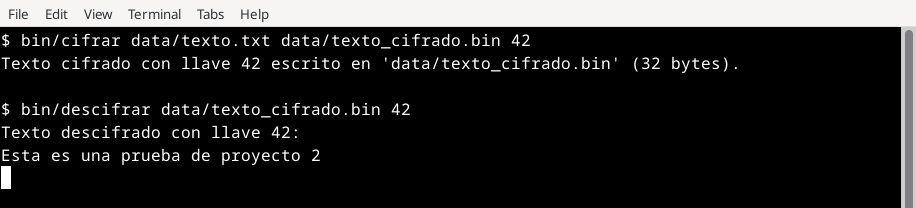
\includegraphics[width=0.7\textwidth]{capturas/b1_cifrar_descifrar.png}
\caption{Ejecución real de \texttt{cifrar} y \texttt{descifrar} con llave 42.}
\label{fig:b1}
\end{figure}

\subsection{Pruebas con \texttt{-np 4} sobre el texto de referencia}
\label{sec:b2}

Se utilizó el texto de referencia del enunciado, \textit{``Esta es una
prueba de proyecto 2''}, buscando la palabra clave \textit{``es una
prueba de''} con el acercamiento naive y 4 procesos MPI.

\subsubsection*{a) Llave 123456}
\begin{lstlisting}[language=bash]
bin/cifrar data/texto.txt data/texto_cifrado.bin 123456
mpirun -np 4 bin/naive_mpi data/texto_cifrado.bin "es una prueba de" 72057594037927935
\end{lstlisting}
\textbf{Resultado medido.} llave encontrada en \textbf{0.094 s} (tiempo
paralelo interno, \texttt{MPI\_Wtime}). La llave cae en el primer
segmento del espacio $[0, 2^{56}-1]$, a unas 123\,456 iteraciones del
inicio del proceso 0.

\subsubsection*{b) Llave 18014398509481983 ($2^{56}/4$, borde entre procesos 0 y 1)}
\begin{lstlisting}[language=bash]
bin/cifrar data/texto.txt data/texto_cifrado.bin 18014398509481983
mpirun -np 4 bin/naive_mpi data/texto_cifrado.bin "es una prueba de" 72057594037927935
\end{lstlisting}
Este caso cae al final del segmento del proceso 0. Es el peor caso
posible para esa llave dentro de su segmento, así que el tiempo de
ejecución se aproxima al de la versión secuencial completa sobre un
cuarto del espacio.

\textbf{Resultado medido.} no termina. Se interrumpió a los 20 s con
\texttt{timeout}, como anticipa el enunciado. El proceso~0 debe recorrer
$2^{54}\approx1.8\times10^{16}$ llaves, que a $3.2\times10^{6}$
llaves/s son unos 180 años.

\subsubsection*{c) Llave 18014398509481984 ($2^{56}/4 + 1$)}
\begin{lstlisting}[language=bash]
bin/cifrar data/texto.txt data/texto_cifrado.bin 18014398509481984
mpirun -np 4 bin/naive_mpi data/texto_cifrado.bin "es una prueba de" 72057594037927935
\end{lstlisting}
Al estar justo al inicio del segmento del proceso 1, este caso produce
un speedup artificialmente alto. El proceso 1 encuentra la llave casi
de inmediato.

\textbf{Resultado medido.} llave encontrada en \textbf{0.031 s}. Un
algoritmo secuencial habría necesitado $2^{56}/4+1$ iteraciones,
así que el speedup aparente es astronómico (y engañoso), tal como
advierte el enunciado.

\textbf{Nota.} en (a), (b) y (c) \texttt{max\_key} es $2^{56}-1$
(72057594037927935) para que el rango se divida en cuatro bloques de
$2^{54}$ llaves.

\subsubsection*{d) Reflexión sobre el comportamiento}

El tiempo observado en el acercamiento naive depende casi
exclusivamente de la posición relativa de la llave solución dentro de
su segmento contiguo, no del tamaño absoluto de \texttt{max\_key}. Si
la llave cae cerca del inicio del segmento de algún proceso, ese
proceso la encuentra rápido y notifica al resto mediante
\texttt{MPI\_Send}. Si cae cerca del final del segmento más largo, el
tiempo total se aproxima al de la búsqueda secuencial sobre ese mismo
segmento. El mismo \texttt{max\_key} puede dar speedups radicalmente
distintos según en qué mitad de qué segmento caiga la solución real.
Esta alta varianza es la motivación central detrás de los tres
acercamientos alternativos descritos a continuación. Todos buscan
reducir la dependencia entre la posición de la llave y el tiempo de
descubrimiento.

El caso (b) no se puede ejecutar completo porque el trabajo total sigue siendo
$O(N)$, y a $3.2\times10^{6}$ llaves/s son años aun con 4 procesos. Por eso
las comparaciones fácil/media/difícil (Sección~\ref{sec:comparativa})
usan un espacio reducido $N_{\text{ef}}=2^{27}$.

\subsection{Acercamientos alternativos}

\subsubsection*{Referencia, acercamiento naive}
\texttt{src/bruteforce/naive\_mpi.c} divide $[0, \texttt{max\_key}]$ en
$np$ segmentos contiguos de igual tamaño. La Figura~\ref{fig:particion}
compara cómo cada acercamiento reparte las llaves entre 4 procesos.

\begin{lstlisting}
Para cada proceso (rank r de np):
  tam   <- (max_key + 1) / np
  inicio <- r * tam ;  fin <- (r == np-1) ? max_key : inicio + tam - 1
  MPI_Irecv(aviso)                       # aviso de "llave encontrada"
  para key desde inicio hasta fin:
    si try_key(key): MPI_Send(key) a los demas; MPI_Cancel(aviso); terminar
    si (key - inicio) % CHECK_INTERVAL == 0 y MPI_Test(aviso): terminar
  si se agoto el segmento: MPI_Wait(aviso)   # espera a quien la tenga
  MPI_Reduce(tiempo maximo, llave) hacia rank 0
\end{lstlisting}

\begin{figure}[H]
\centering
\resizebox{0.9\textwidth}{!}{\begin{tikzpicture}[x=1cm, y=0.8cm]
  \tikzset{cell/.style={draw, minimum height=0.5cm, inner sep=0pt, font=\scriptsize, anchor=west}}
  \node[anchor=east, font=\small] at (-0.2,0) {Naive};
  \foreach \i/\c in {0/blue!25, 1/green!25, 2/orange!30, 3/red!25}
     \node[cell, fill=\c, minimum width=3.9cm] at (\i*3.9,0) {P\i\ bloque contiguo};
  \node[anchor=east, font=\small] at (-0.2,-1) {Striding};
  \foreach \i/\p/\c in {0/0/blue!25,1/1/green!25,2/2/orange!30,3/3/red!25,4/0/blue!25,5/1/green!25,6/2/orange!30,7/3/red!25,8/0/blue!25,9/1/green!25,10/2/orange!30,11/3/red!25,12/0/blue!25,13/1/green!25,14/2/orange!30,15/3/red!25}
     \node[cell, fill=\c, minimum width=0.975cm] at (\i*0.975,-1) {P\p};
  \node[anchor=east, font=\small] at (-0.2,-2) {Shuffled};
  \foreach \i/\c in {0/blue!25, 1/green!25, 2/orange!30, 3/red!25}
     \node[cell, fill=\c, minimum width=3.9cm] at (\i*3.9,-2) {P\i\ $(a\cdot idx+b)\bmod N$};
  \node[anchor=east, font=\small] at (-0.2,-3) {Master-worker};
  \foreach \i/\p/\c in {0/1/blue!25,1/2/green!25,2/3/orange!30,3/1/blue!25,4/2/green!25,5/3/orange!30,6/2/green!25,7/1/blue!25,8/3/orange!30,9/2/green!25,10/1/blue!25,11/3/orange!30}
     \node[cell, fill=\c, minimum width=1.3cm] at (\i*1.3,-3) {W\p};
  \node[anchor=east, font=\small] at (-0.2,-4) {H\'ibrido};
  \foreach \i/\c in {0/blue!25, 1/green!25, 2/orange!30, 3/red!25}
     \node[cell, fill=\c, minimum width=3.9cm] at (\i*3.9,-4) {P\i\ bloque $\to$ hilos};
\end{tikzpicture}}
\caption{Reparto del espacio de llaves $[0, N-1]$ (de izquierda a derecha) entre 4 procesos.
Cada color es un proceso (en master-worker, un trabajador; el rank 0 solo coordina).
En striding los colores se alternan llave a llave; en master-worker, bloque a bloque y bajo demanda;
en shuffled cada bloque contiguo de \'indices se dispersa por todo el espacio.}
\label{fig:particion}
\end{figure}

\subsubsection{Acercamiento 1 --- Master-Worker dinámico}
\label{sec:masterworker}

\textbf{Archivo.} \texttt{src/bruteforce/master\_worker\_mpi.c}

El proceso de rank 0 actúa exclusivamente como maestro y no participa
en la búsqueda. Distribuye bloques pequeños de tamaño
\texttt{chunk\_size} (por defecto, 50{,}000 llaves) a los procesos
trabajadores (\texttt{rank} $\geq 1$) bajo demanda. Cuando un
trabajador termina de recorrer su bloque sin encontrar la llave, pide
el siguiente al maestro. Esta estrategia de \textit{pull} elimina la
varianza observada en el acercamiento naive, porque ningún proceso
queda permanentemente atado a un segmento desfavorablemente largo. En
cuanto un proceso libera capacidad, se le asigna más trabajo.

\begin{lstlisting}[frame=single, basicstyle=\ttfamily\footnotesize]
Maestro (rank=0):              Trabajador (rank>=1):
  reparte bloque inicial  -->    recibe [inicio, fin]
  loop:                          loop:
    recibe resultado       <--     busca en [inicio, fin]
    si llave hallada:              envia resultado
      envia TAG_STOP a todos -->   si TAG_STOP: termina
    si hay mas trabajo:            si TAG_WORK: repite
      envia TAG_WORK         -->
\end{lstlisting}

El costo de esta estrategia es el overhead de comunicación. Cada
bloque consumido implica una ronda adicional de mensajes
maestro-trabajador, lo que puede volverse significativo si
\texttt{chunk\_size} es muy pequeño en relación con la latencia de red.

\begin{lstlisting}[language=bash]
mpirun -np 4 bin/master_worker_mpi data/texto_cifrado.bin "es una prueba de" <max_key> [chunk_size]
\end{lstlisting}

Las ejecuciones reales de los 5 acercamientos (incluyendo este) sobre
el mismo caso de prueba se muestran juntas en la
Figura~\ref{fig:b3todos}, al final de esta subsección.

\subsubsection{Acercamiento 2 --- Intercalado / Striding}

\textbf{Archivo.} \texttt{src/bruteforce/striding\_mpi.c}

En lugar de un bloque contiguo, cada proceso de rank $r$ recorre las
llaves $r, r+np, r+2\cdot np, \dots$, donde $np$ es el número total de
procesos. De esta forma, todos los procesos exploran simultáneamente
la misma ``profundidad relativa'' del espacio de búsqueda en todo
momento. Esto elimina por completo la correlación entre la posición
absoluta de la llave solución y qué proceso tiene ventaja. Sin
importar dónde caiga la llave, en promedio todos los procesos llevan
un avance similar cuando se encuentra.

\begin{lstlisting}[frame=single, basicstyle=\ttfamily\footnotesize]
Para cada proceso (rank r de np):
  key <- r
  mientras key <= max_key:
    si try_key(key): avisar a los demas y terminar
    si (key - r) % CHECK_INTERVAL == 0: revisar aviso (MPI_Test)
    key <- key + np        # salto de tamano np: entrelazado
\end{lstlisting}

\begin{lstlisting}[language=bash]
mpirun -np 4 bin/striding_mpi data/texto_cifrado.bin "es una prueba de" <max_key>
\end{lstlisting}

Ver Figura~\ref{fig:b3todos}.

\subsubsection{Acercamiento 3 --- Partición contigua con shuffle pseudo-aleatorio}

\textbf{Archivo.} \texttt{src/bruteforce/shuffled\_mpi.c}

Este acercamiento conserva la misma partición en bloques contiguos que
el naive (y, por tanto, la misma simplicidad de asignación estática de
trabajo), pero en lugar de recorrer cada bloque en orden ascendente,
cada índice lógico \texttt{idx} dentro del bloque se mapea a la llave
real mediante una función de congruencia lineal.
\[
\texttt{key}(\texttt{idx}) = (a \cdot \texttt{idx} + b) \bmod N
\]
donde $N = \texttt{max\_key} + 1$ y $a$ se elige coprimo con $N$. Esta
construcción garantiza una biyección sobre $[0, N-1]$ y cada llave del
espacio se visita exactamente una vez en total. Pero el \emph{orden}
en que cada proceso las visita queda ``barajado'' de forma determinista
y reproducible. No es una permutación aleatoria real, sino
pseudo-aleatoria vía aritmética modular. El efecto práctico es similar
al striding, rompe la correlación entre posición y tiempo de hallazgo,
pero sin necesitar que los procesos avancen en sincronía por todo el
espacio.

\begin{lstlisting}[frame=single, basicstyle=\ttfamily\footnotesize]
N <- max_key + 1
[idx_start, idx_end] <- segmento contiguo del proceso (igual que naive)
para idx desde idx_start hasta idx_end:
  key <- (a * idx + b) mod N      # biyeccion pseudo-aleatoria
  si try_key(key): avisar a los demas y terminar
  cada CHECK_INTERVAL: revisar aviso (MPI_Test)
\end{lstlisting}

\begin{lstlisting}[language=bash]
mpirun -np 4 bin/shuffled_mpi data/texto_cifrado.bin "es una prueba de" <max_key>
\end{lstlisting}

Ver Figura~\ref{fig:b3todos}.

\subsubsection{Acercamiento 4 --- Híbrido MPI + OpenMP}

\textbf{Archivo.} \texttt{src/bruteforce/hybrid\_mpi\_omp.c}

Esta versión combina memoria distribuida (MPI) con memoria compartida
dentro de cada nodo (OpenMP, OpenMP ARB, 2021)\footnote{\url{https://www.openmp.org/specifications/}.}. Añade un segundo nivel
de paralelismo dentro de cada proceso MPI. El bloque contiguo asignado
a cada proceso se subdivide entre los hilos de OpenMP disponibles,
cada uno recorriendo su sub-bloque con un stride igual al número de
hilos. Es el mismo principio de striding, aplicado ahora a nivel de
hilos en memoria compartida en vez de a nivel de procesos en memoria
distribuida. MPI se inicializa con \texttt{MPI\_Init\_thread}
solicitando el nivel \texttt{MPI\_THREAD\_FUNNELED}, ya que únicamente
el hilo maestro (\texttt{omp} thread 0) de cada proceso realiza
llamadas a funciones MPI. El resto de los hilos se limitan a ejecutar
\texttt{try\_key} en su porción del espacio de búsqueda.

El objetivo de este acercamiento es doble. Primero, reducir el número
de procesos MPI necesarios para saturar los núcleos de una máquina,
disminuyendo así el overhead de paso de mensajes. Segundo, aprovechar
la memoria compartida dentro de cada nodo para comunicar el estado de
``llave encontrada'' entre hilos de forma más económica que mediante
mensajes MPI.

\begin{lstlisting}[frame=single, basicstyle=\ttfamily\footnotesize]
Nivel 1 (por proceso MPI, rank r de np):
  [block_start, block_end] <- segmento contiguo (igual que naive)
  encontrado_local <- bandera compartida entre hilos (false)

  Nivel 2 (por hilo OpenMP, id t de nthreads), en paralelo:
    key <- block_start + t
    mientras key <= block_end y no encontrado_local:
      si try_key(key): encontrado_local <- true; guardar key; salir
      si t == 0 y toca revisar: sondear aviso MPI (MPI_Test)
      key <- key + nthreads          # entrelazado entre hilos

  (fin de la region paralela, los hilos se unen)
  si encontrado_local (hallado por este proceso):
    avisar a los demas procesos (MPI_Send)
  si no: esperar aviso de otro proceso (MPI_Wait)
\end{lstlisting}

\begin{lstlisting}[language=bash]
mpirun -np 4 bin/hybrid_mpi_omp data/texto_cifrado.bin "es una prueba de" <max_key> [nthreads]
\end{lstlisting}

Ver Figura~\ref{fig:b3todos}.

\begin{figure}[H]
\centering
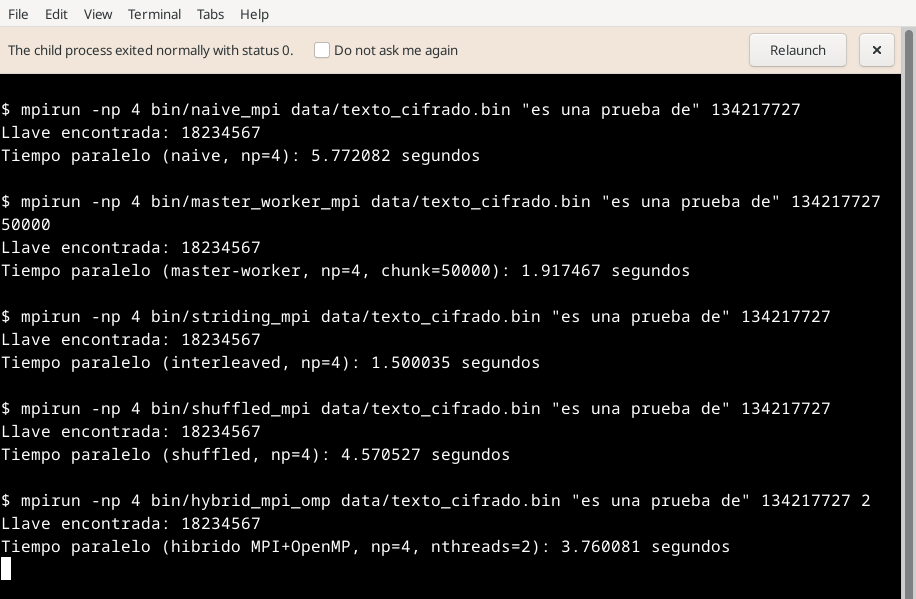
\includegraphics[width=0.85\textwidth]{capturas/b3_acercamientos.png}
\caption{Ejecución real de los 5 acercamientos paralelos sobre el mismo
caso de prueba (llave objetivo = 18{,}234{,}567, \texttt{max\_key} =
134{,}217{,}727, $np=4$). Los 5 encuentran exactamente la llave
correcta de forma consistente.}
\label{fig:b3todos}
\end{figure}

\subsection{Comparativa de tiempos (fácil / media / difícil)}
\label{sec:comparativa}

Siguiendo la metodología del enunciado, se definieron tres llaves
(fácil, media y difícil) con las mismas fracciones propuestas pero
aplicadas sobre un espacio efectivo reducido $N_{\text{ef}}=2^{27}$ (ver
Sección~\ref{sec:secuencial}). \textbf{El espacio de búsqueda es el
mismo para los tres casos} ($\texttt{max\_key}=2^{27}-1$), de modo que
lo único que cambia es la posición de la llave, tal como plantea el
enunciado. Se ejecutó cada uno de los seis programas (secuencial + 5
paralelos) con $np=4$ y, para el híbrido, 2 hilos por proceso (8
hilos en total). Los tiempos son los que imprime cada programa
(\texttt{MPI\_Wtime} o reloj interno), es decir, el tiempo de búsqueda
sin el arranque de \texttt{mpirun}. El tiempo de pared del comando
completo se conserva en la columna \texttt{tiempo\_wall\_segundos} del
CSV; difiere en $\approx1.5$\,s por el lanzamiento de MPI. Cada punto
es una sola corrida (no hay repeticiones). Los resultados completos
están en el Anexo~\ref{sec:anexo2} y en
\texttt{resultados\_benchmark.csv}.

Con $np=4$ y bloques de $2^{27}/4$ llaves, la llave fácil es la primera del
bloque del proceso~2, la media está a la mitad de ese bloque y la
difícil ($\approx0.22N$) al 88\,\% del bloque del proceso~0.

\begin{table}[H]
\centering
\small
\begin{tabular}{lcccccc}
\toprule
\textbf{Caso} & \textbf{Secuencial} & \textbf{Naive} & \textbf{Master-W.} & \textbf{Striding} & \textbf{Shuffled} & \textbf{Híbrido} \\
\midrule
Base (123\,456) & 0.039 & 0.156 & 0.016 & 0.063 & 7.903 & 0.125 \\
Fácil           & 20.890 & 0.094 & 6.934 & 5.270 & 0.878 & 0.154 \\
Media           & 26.097 & 5.299 & 8.640 & 6.594 & 3.286 & 2.724 \\
Difícil         & 9.197  & 9.244 & 3.078 & 2.364 & 8.761 & 4.696 \\
\bottomrule
\end{tabular}
\caption{Tiempo de búsqueda (s) por caso y acercamiento, $np=4$,
espacio fijo $2^{27}$ (\texttt{hybrid\_mpi\_omp} con 2 hilos por
proceso). Fuente en \texttt{resultados\_benchmark.csv}.}
\label{tab:comparativa}
\end{table}

\begin{table}[H]
\centering
\small
\begin{tabular}{p{2.6cm}p{3.6cm}p{3.6cm}p{3.5cm}}
\toprule
\textbf{Acercamiento} & \textbf{Speedup (fácil / media / difícil)} & \textbf{Eficiencia (fácil / media / difícil)} & \textbf{Divisor de eficiencia} \\
\midrule
Naive           & 222.9 / 4.92 / 0.99 & 55.7 / 1.23 / 0.25 & $np=4$ \\
Master-worker   & 3.01 / 3.02 / 2.99  & 0.75 / 0.76 / 0.75 & $np=4$ \\
Striding        & 3.96 / 3.96 / 3.89  & 0.99 / 0.99 / 0.97 & $np=4$ \\
Shuffled        & 23.8 / 7.94 / 1.05  & 5.9 / 1.99 / 0.26  & $np=4$ \\
Híbrido (2 hilos) & 135.7 / 9.58 / 1.96 & 17.0 / 1.20 / 0.25 & $np\times$hilos $=8$ \\
\bottomrule
\end{tabular}
\caption{Speedup ($T_{seq}/T_{par}$) y eficiencia (speedup dividido
entre las unidades de cómputo) respecto a la versión secuencial
(calculado con \texttt{scripts/speedup.py}).}
\label{tab:speedup}
\end{table}

\subsubsection*{Modelo analítico del tiempo paralelo}
\label{sec:modelo}

Los resultados se pueden predecir sin ejecutar nada. Sea $k$ la llave,
$N$ el tamaño del espacio, $p$ el número de procesos, $B=N/p$ el tamaño
del bloque y $r\approx3.21\times10^{6}$ llaves/s la tasa medida de un
núcleo (Tabla~\ref{tab:secuencial}). El tiempo paralelo es el del
proceso que encuentra la llave, es decir, las iteraciones que le toca
hacer hasta llegar a ella, divididas entre $r$.

\begin{center}
\small
\begin{tabular}{lll}
\toprule
\textbf{Acercamiento} & \textbf{Iteraciones hasta hallar $k$} & \textbf{Speedup} \\
\midrule
Secuencial & $k+1$ & $1$ \\
Naive & $k-\lfloor k/B\rfloor B+1$ (posición dentro de su bloque) & $\dfrac{k+1}{k-\lfloor k/B\rfloor B+1}$, entre $1$ y $\approx k$ \\
Striding & $\approx k/p$ (todos avanzan al mismo ritmo) & $\approx p$ \\
Master-worker & $\approx k/(p-1)$ (el maestro no busca) & $\approx p-1$ \\
Shuffled & $idx-\lfloor idx/B\rfloor B+1$, con $idx=a^{-1}(k-b)\bmod N$ & depende de $idx$ \\
\bottomrule
\end{tabular}
\end{center}

La Tabla~\ref{tab:modelo} compara este modelo con las mediciones
(las llaves de naive y shuffled se calcularon con los mismos $a$ y
$b$ que usa el programa).

\begin{table}[H]
\centering
\small
\begin{tabular}{lcccccccc}
\toprule
 & \multicolumn{2}{c}{\textbf{Naive}} & \multicolumn{2}{c}{\textbf{Striding}} & \multicolumn{2}{c}{\textbf{Master-W.}} & \multicolumn{2}{c}{\textbf{Shuffled}} \\
\textbf{Caso} & pred. & med. & pred. & med. & pred. & med. & pred. & med. \\
\midrule
Base    & 0.038 & 0.156 & 0.010 & 0.063 & 0.013 & 0.016 & 7.81 & 7.90 \\
Fácil   & $\approx0$ & 0.094 & 5.23 & 5.27 & 6.97 & 6.93 & 0.80 & 0.88 \\
Media   & 5.23 & 5.30 & 6.53 & 6.59 & 8.71 & 8.64 & 3.19 & 3.29 \\
Difícil & 9.19 & 9.24 & 2.30 & 2.36 & 3.06 & 3.08 & 8.64 & 8.76 \\
\bottomrule
\end{tabular}
\caption{Tiempo paralelo predicho por el modelo vs. medido (s), $np=4$, $N=2^{27}$.}
\label{tab:modelo}
\end{table}

Las predicciones coinciden con lo medido (diferencias de $\approx$1--3\,\%
cuando el tiempo es de varios segundos). Los desvíos en las filas de
tiempos muy pequeños (naive 0.038 vs. 0.156) son un costo fijo de
$\approx0.1$\,s de aviso y cierre entre procesos
(\texttt{MPI\_Send}/\texttt{MPI\_Wait}), que el modelo no incluye. Esto
significa que los resultados no son casualidad ni ruido, están
determinados por la posición de la llave. El híbrido sigue el mismo modelo con la mitad
del tiempo de naive (2 hilos por bloque): predice 2.6\,s en media y 4.6\,s en
difícil, y se midió 2.7\,s y 4.7\,s.

\paragraph{Qué implica para el tiempo paralelo esperado.} Si la llave es
uniforme en $[0,N)$, la posición dentro del bloque de naive es uniforme
en $[0,B)$, así que su tiempo esperado es $B/2=N/(2p)$ iteraciones. El de
striding es $E[k]/p=N/(2p)$. \textbf{Los dos tienen el mismo tiempo
esperado y el mismo peor caso ($N/p$)}. Lo que cambia es la dispersión
del speedup. Naive depende de la posición (de $\approx1$ a $\approx k$),
mientras que striding da $\approx p$ siempre. Master-worker tiene un
tiempo esperado peor en un factor $p/(p-1)$ en una sola máquina
homogénea, y su ventaja (balancear nodos de distinta velocidad) no se
midió. Shuffled convierte el speedup de naive en una variable
pseudo-aleatoria sin mejorar su valor medio.

Observaciones sobre la Tabla~\ref{tab:speedup}.

\begin{itemize}
    \item \textbf{Naive} va de 222.9 a 0.99 según dónde caiga la llave,
    exactamente el fenómeno del enunciado. Su eficiencia $>1$ es suerte
    posicional, no ganancia paralela.
    \item \textbf{Striding} es el único consistente, con $\approx np$ (3.96,
    3.96, 3.89) sin importar la llave. A cambio nunca tiene el golpe de
    suerte de naive (en el caso fácil, 5.27\,s vs. 0.094\,s).
    \item \textbf{Master-worker} rinde $np-1\approx3.0$ porque el rank~0 sólo
    coordina. El costo de los mensajes (un bloque de 50\,000 llaves son
    $\approx16$\,ms de cómputo) es pequeño frente a esa pérdida.
    \item \textbf{Shuffled} no elimina la varianza, la aleatoriza (23.8,
    7.94 y 1.05; con la llave base tarda 7.9\,s, unas 200 veces más que la
    secuencial).
    \item \textbf{Híbrido} conserva los bloques contiguos de naive (135.7,
    9.58, 1.96) pero con 2 hilos por bloque, así que su tiempo es la mitad del
    de naive en media y difícil (Sección~\ref{sec:hilos}).
\end{itemize}

\begin{figure}[H]
\centering
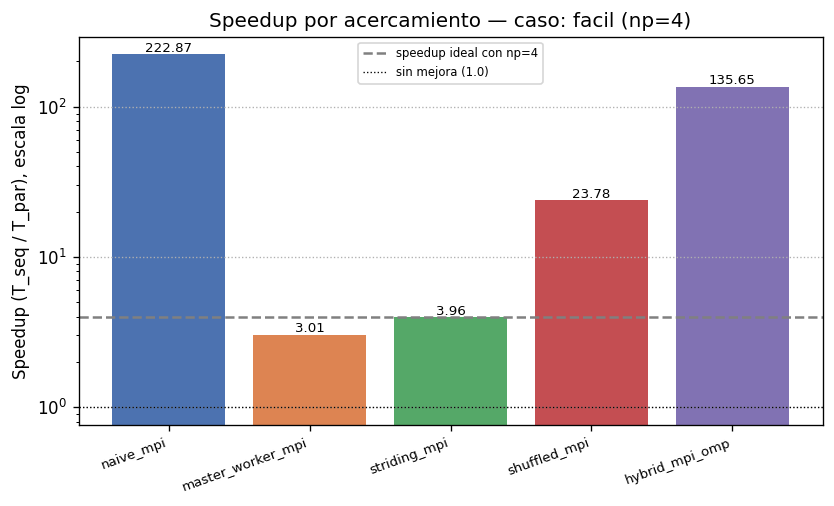
\includegraphics[width=0.32\textwidth]{../results/speedup_facil.png}
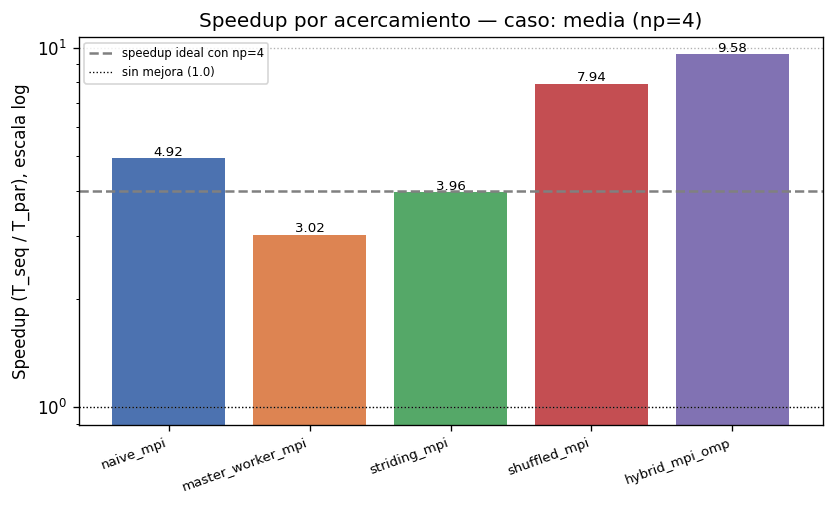
\includegraphics[width=0.32\textwidth]{../results/speedup_media.png}
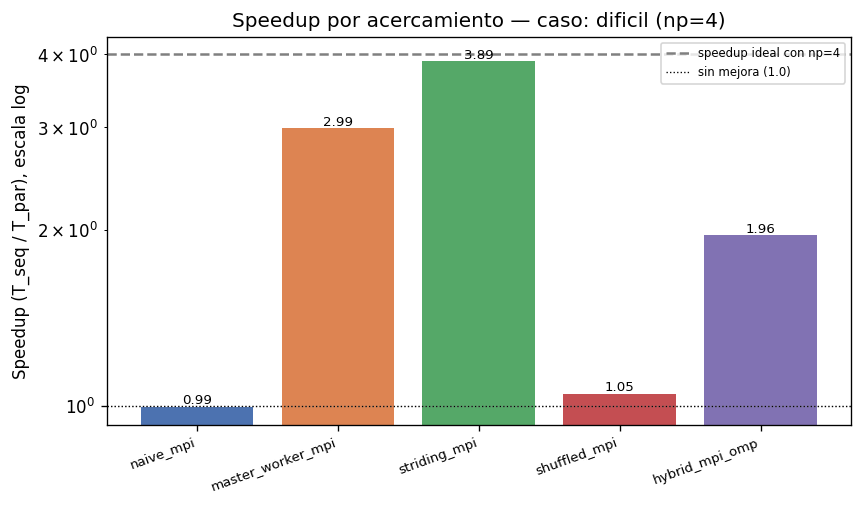
\includegraphics[width=0.32\textwidth]{../results/speedup_dificil.png}
\caption{Speedup por acercamiento (escala log), $np=4$, para los casos fácil, media y difícil.}
\label{fig:speedup}
\end{figure}

\subsubsection*{Experimento con llaves aleatorias}
\label{sec:random}

Tres llaves no bastan para estimar el tiempo esperado. Se repitió la
comparación con 30 llaves aleatorias uniformes en $[0, N-1]$ (una por cada
uno de 30 estratos iguales, semilla fija 42), con $np=4$ y el híbrido con
2 hilos. Para que quepa en unos 7 minutos se usó $N=2^{24}$ en lugar de
$2^{27}$ (misma tasa de $3.2\times10^{6}$ llaves/s, tiempos 8 veces menores).
Las llaves y los tiempos están en \texttt{resultados\_random.csv}, y se
generan con \texttt{scripts/random\_keys.sh} y \texttt{scripts/random\_summary.py}.

\begin{table}[H]
\centering
\small
\begin{tabular}{lrrrrrrr}
\toprule
\textbf{Acercamiento} & $\bar T_{seq}/\bar T$ & \textbf{Media} & \textbf{Mediana} & \textbf{Máx.} & \textbf{Desv.} & \textbf{Speedup mín.} & \textbf{Speedup máx.} \\
\midrule
Secuencial        & 1.00 & 2.61 & 2.63 & 5.09 & 1.54 & 1.00 & 1.00 \\
Naive             & 3.51 & 0.74 & 0.72 & 1.31 & 0.38 & 0.38 & 42.2 \\
Master-worker     & 2.99 & 0.87 & 0.88 & 1.69 & 0.52 & 2.89 & 3.16 \\
Striding          & 3.63 & 0.72 & 0.73 & 1.32 & 0.38 & 0.76 & 3.86 \\
Shuffled          & 4.04 & 0.64 & 0.55 & 1.33 & 0.41 & 0.25 & 32.5 \\
Híbrido (2 hilos) & 5.45 & 0.48 & 0.50 & 0.81 & 0.21 & 0.32 & 16.9 \\
\bottomrule
\end{tabular}
\caption{Tiempo de búsqueda (s) con 30 llaves aleatorias, $N=2^{24}$, $np=4$. $\bar T_{seq}/\bar T$ es la razón de tiempos medios. El modelo de la Sección~\ref{sec:modelo} predice medias de 2.63\,s (secuencial), 0.66\,s (naive y striding) y 0.88\,s (master-worker).}
\label{tab:random}
\end{table}

\begin{figure}[H]
\centering
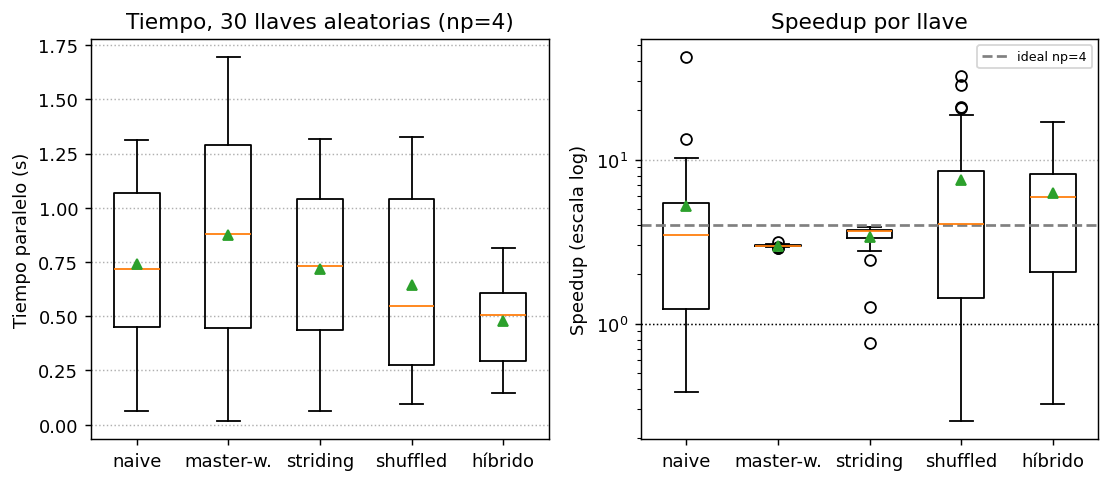
\includegraphics[width=\textwidth]{../results/variabilidad_random.png}
\caption{Distribución del tiempo y del speedup con 30 llaves aleatorias (cajas, la marca es la media; speedup en escala log).}
\label{fig:variabilidad}
\end{figure}

\begin{itemize}
    \item \textbf{El modelo acierta en las medias.} Secuencial 2.61 vs. 2.63\,s, master-worker 0.87 vs. 0.88\,s, naive y striding 0.74 y 0.72 vs. 0.66\,s (la diferencia es el costo fijo de aviso, $\approx0.07$\,s). Naive y striding tienen el mismo tiempo esperado, como predice la teoría, ya que la diferencia de 0.02\,s es menor que el error estándar ($\approx0.07$\,s).
    \item \textbf{La dispersión del tiempo no distingue a los acercamientos.} El coeficiente de variación del tiempo es 0.4--0.6 en todos, porque el tiempo es proporcional a la posición de una llave uniforme. Lo que sí los distingue es la dispersión del \textit{speedup}. Naive va de 0.38 a 42.2 y shuffled de 0.25 a 32.5, striding de 0.76 a 3.86 y master-worker de 2.89 a 3.16. En striding el mínimo menor que 1 aparece sólo con llaves tan pequeñas que la corrida dura menos de 0.2\,s y domina el costo fijo.
    \item \textbf{Shuffled no es mejor que naive en tiempo esperado.} Su media es 0.64 vs. 0.74\,s, diferencia de alrededor de un error estándar, indistinguible con 30 llaves.
    \item \textbf{El híbrido tiene el menor tiempo medio} (0.48\,s frente a 0.74\,s de naive, el 65\,\%). Usa 8 hilos, así que su eficiencia es $5.45/8\approx0.68$, frente a 0.88 de naive y 0.91 de striding con 4 procesos.
\end{itemize}

\subsubsection*{Escalado del híbrido con los hilos}
\label{sec:hilos}

Con $np=1$ y la llave difícil, el híbrido es OpenMP puro dentro de un bloque. La
Figura~\ref{fig:hilos} (izquierda) compara tres configuraciones
(\texttt{scripts/hybrid\_threads.sh}, datos en \texttt{resultados\_hybrid\_threads.csv}).
Con el binding por defecto de Open MPI 5, el proceso queda atado a un solo núcleo
físico (2 hilos de hardware) y el tiempo se estanca en $\approx5.9$\,s ($1.55\times$)
con 2 a 20 hilos. Lanzando con \texttt{--bind-to none} el escalado es casi lineal:
1.99$\times$ con 2 hilos, 3.93$\times$ con 4, 7.7$\times$ con 8, 11.7$\times$ con 16 y
14.2$\times$ con 20. Pasado 8 hilos se aplana, lo esperable en un i5-14600KF (6 núcleos
P con SMT y 8 núcleos E, más lentos). Striding con $T$ procesos MPI da lo mismo, así que
hilos y procesos son equivalentes dentro de un nodo. A la derecha, con $T=8$ y 8 llaves
consecutivas (cada una la posee un hilo distinto), el tiempo varía entre 1.16 y
1.54\,s. Con reparto estático, el tiempo lo fija el núcleo en que corre el hilo
propietario de la llave.

\begin{figure}[H]
\centering
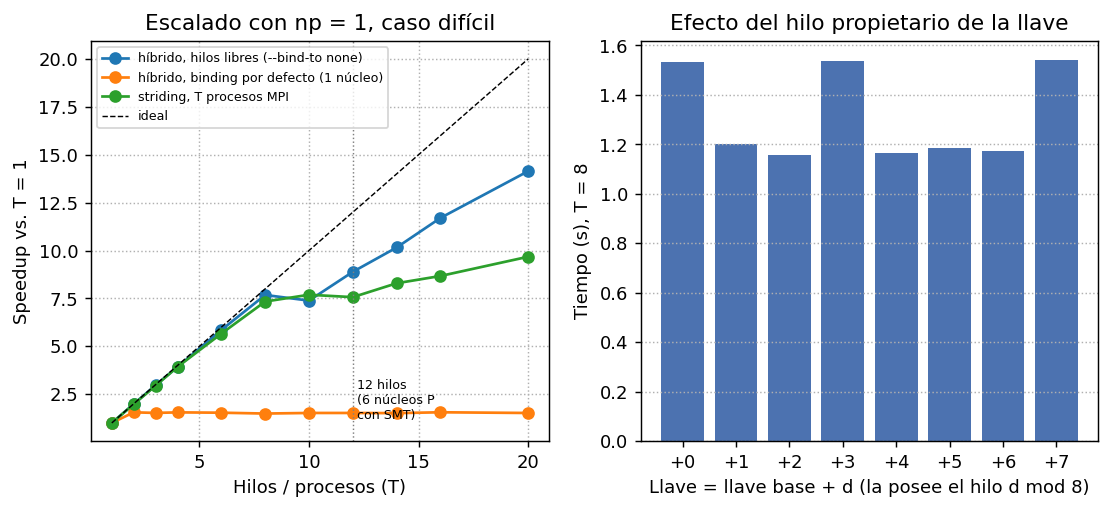
\includegraphics[width=\textwidth]{../results/hybrid_hilos.png}
\caption{Escalado del híbrido con los hilos ($np=1$, caso difícil) y efecto del hilo propietario.}
\label{fig:hilos}
\end{figure}

Para ver si conviene más procesos o más hilos, se repartieron 8 unidades de cómputo de
cuatro formas sobre las mismas 30 llaves aleatorias ($N=2^{24}$, \texttt{scripts/hybrid\_grid.sh}).
El modelo predice el mismo tiempo medio ($N/16$ iteraciones, 0.33\,s) para todas.

\begin{table}[H]
\centering
\small
\begin{tabular}{lrrrrr}
\toprule
\textbf{Procesos $\times$ hilos} & \textbf{Media} & \textbf{Mediana} & \textbf{Máx.} & $\bar T_{seq}/\bar T$ & \textbf{Eficiencia} \\
\midrule
$8\times1$ (naive) & 0.490 & 0.533 & 0.731 & 5.31 & 0.66 \\
$4\times2$ & 0.486 & 0.445 & 0.823 & 5.36 & 0.67 \\
$2\times4$ & 0.428 & 0.416 & 0.813 & 6.09 & 0.76 \\
$1\times8$ & 0.367 & 0.361 & 0.721 & 7.09 & 0.89 \\
\bottomrule
\end{tabular}
\caption{Tiempo (s) con 8 unidades de cómputo repartidas de distinta forma, 30 llaves aleatorias.}
\label{tab:grid}
\end{table}

\begin{figure}[H]
\centering
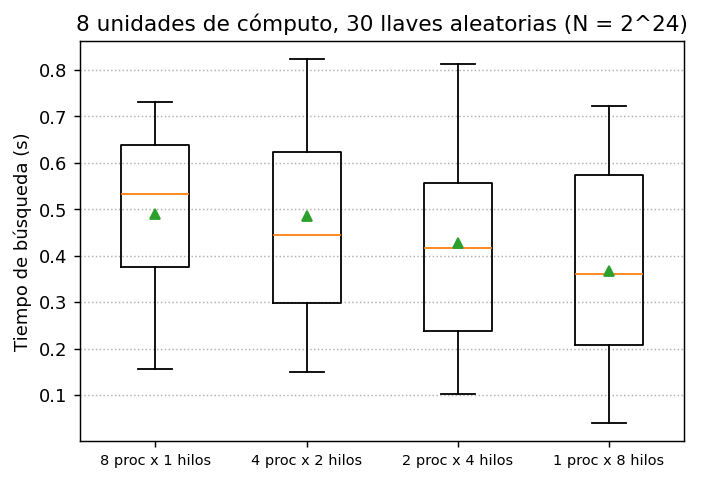
\includegraphics[width=0.6\textwidth]{../results/hybrid_grid.png}
\caption{Distribución del tiempo con 8 unidades de cómputo repartidas entre procesos e hilos.}
\label{fig:grid}
\end{figure}

Menos procesos y más hilos es mejor (0.37 vs. 0.49\,s), porque hay menos mensajes MPI y
sondeos, y $1\times8$ además tiene un speedup consistente (1.22 a 7.77, sin bloques que
dependan de la posición de la llave).

% =======================================================================
\section{Discusión, conclusiones y recomendaciones}
% =======================================================================

\subsection*{Retos encontrados y lecciones aprendidas}

El reto técnico más significativo no estuvo en la paralelización en
sí, sino en la representación de la llave. DES ignora el bit de paridad
de cada byte, así que los 56 bits de la llave numérica se empaquetan a
razón de 7 por byte para que cada valor corresponda a una llave DES
distinta (Sección~\ref{sec:des-wrapper}). En un bruteforce conviene
verificar esa correspondencia uno a uno antes de medir tiempos.

El segundo reto fue de escala. El enunciado define los casos
fácil/media/difícil como fracciones de $2^{56}$, pero a la tasa de
verificación medida en esta máquina esas fracciones representan años
de cómputo, incluso paralelizadas. Esto llevó a sustituir $2^{56}$ por
un espacio efectivo reducido ($N_{\text{ef}} = 2^{27}$) que preserva
el fenómeno de interés, la posición relativa dentro del segmento, con
tiempos de ejecución manejables (Sección~\ref{sec:secuencial}). Es una
decisión de diseño experimental, no un atajo que invalide el análisis.

El tercer reto fue el diseño de las pruebas. El espacio de búsqueda debe
ser el mismo en todos los casos y variar sólo la posición de la llave, y
el tiempo debe medirse dentro del programa (el arranque de
\texttt{mpirun} añade $\approx1.5$\,s al tiempo de pared).

Por último, se aprendió que con un texto de prueba y palabra clave tan
cortos, un descifrado con la llave incorrecta puede, por azar,
contener la palabra clave buscada. Eso sería un falso positivo. No se
observó en la práctica en las corridas finales reportadas en este
informe, pero es una limitación real del criterio de validación por
\textit{substring}. Vale la pena mencionarla para cualquier extensión
futura del proyecto, por ejemplo usando una frase clave más larga o
verificando un segundo criterio de coincidencia.

\begin{itemize}
    \item \textbf{Varianza del naive, teoría y evidencia.} El caso
    analítico de la Sección~\ref{sec:b2} lo muestra en el extremo. Con
    $np=4$ y $2^{56}$ llaves, la misma \texttt{max\_key} da un speedup de
    $\approx1$ si la llave está al final del bloque del proceso~0 y de
    $\approx4.5\times10^{15}$ si está al inicio del bloque del
    proceso~1. Los casos medidos a escala $2^{27}$ lo confirman, ya que naive
    va de 222.9 a 0.99 (coeficiente de variación del speedup entre los
    tres casos, 1.36). Striding, en cambio, da 3.96, 3.96 y 3.89
    (CV 0.01). Con tres llaves el CV es ilustrativo, así que se
    repitió con 30 llaves aleatorias (Sección~\ref{sec:random}).
    \item \textbf{Tiempo esperado y consistencia (Secciones~\ref{sec:modelo} y~\ref{sec:random}).}
    Con 30 llaves aleatorias, naive y striding tienen el mismo tiempo medio
    (0.74 y 0.72\,s), como predice el modelo ($N/2p$ iteraciones), y el
    mismo peor caso. La mejora de striding es de \textit{consistencia}, ya que su speedup
    queda entre 0.76 y 3.86 (el mínimo menor que 1 es costo fijo en llaves
    diminutas) frente a 0.38--42.2 de naive. Master-worker es consistente
    pero rinde $np-1$. Shuffled aleatoriza el speedup (0.25--32.5) sin
    mejorar la media. Si se busca predecibilidad, striding es la mejor
    opción medida; si se busca el menor tiempo medio, el híbrido con 2 hilos
    (0.48\,s), aunque usa 8 hilos en lugar de 4 procesos.
    \item \textbf{Overhead de comunicación.} Master-worker envía un
    mensaje por bloque, pero su speedup de $\approx3.0$ se explica por
    tener un núcleo menos buscando. Con un \texttt{chunk\_size} mucho
    menor o más latencia podría pesar más; no se midió.
    \item \textbf{Beneficio del híbrido (Sección~\ref{sec:hilos}).} Con los hilos libres
    escala casi linealmente hasta 8 hilos (7.7$\times$) y, con las mismas 8 unidades de
    cómputo, 1 proceso $\times$ 8 hilos es más rápido que 8 procesos (0.37 vs. 0.49\,s de media)
    por tener menos comunicación. Un hallazgo práctico es que Open MPI 5 ata cada
    proceso a un solo núcleo por defecto, y los hilos de OpenMP compartían ese
    núcleo (speedup de sólo $\approx1.55\times$ sin importar cuántos hilos). Se
    corrigió lanzando con \texttt{--bind-to none}.
    \item \textbf{Recomendación.} Para trabajo futuro, valdría la pena
    extender las pruebas a un cluster MPI de 2+ máquinas físicas (ver
    extras del enunciado), para observar cómo se comportan estos
    mismos acercamientos cuando la comunicación deja de ser intra-nodo
    y pasa a depender de la latencia de una red local real.
\end{itemize}

En conclusión, el programa base funciona correctamente de principio a
fin. Recibe el texto plano desde archivo, lo cifra con una llave
arbitraria pasada por parámetro, y las seis variantes de búsqueda
(secuencial y cinco paralelas) recuperan exactamente esa misma llave,
sin colisiones ni falsos positivos.
Todas imprimen la llave encontrada, el archivo de entrada y la palabra
clave usada en cada corrida (Secciones~\ref{sec:b1}
y~\ref{sec:comparativa}).

% =======================================================================
\section{Anexo 1 --- Catálogo de funciones y librerías}
\label{sec:anexo1}
% =======================================================================

\subsubsection*{\texttt{des\_encrypt} --- \texttt{src/common/des.c}}
\small\texttt{void des\_encrypt(long key, unsigned char *buf, size\_t len)}\normalsize
\begin{itemize}[nosep]
    \item \textbf{Entradas.} \texttt{key} (long, $0$ a $2^{56}-1$), \texttt{buf} (buffer a cifrar, múltiplo de 8 B), \texttt{len} (tamaño en bytes).
    \item \textbf{Salidas.} Modifica \texttt{buf} in-place (cifrado DES en modo ECB).
    \item \textbf{Descripción.} Convierte \texttt{key} a un bloque de 8 bytes, invoca \texttt{DES\_set\_key\_unchecked} y \texttt{DES\_ecb\_encrypt} de OpenSSL sobre cada bloque de 8 bytes del buffer.
\end{itemize}

\subsubsection*{\texttt{des\_decrypt} --- \texttt{src/common/des.c}}
\small\texttt{void des\_decrypt(long key, unsigned char *buf, size\_t len)}\normalsize
\begin{itemize}[nosep]
    \item Idéntica a \texttt{des\_encrypt}, pero invoca \texttt{DES\_ecb\_encrypt} con el flag \texttt{DES\_DECRYPT}.
\end{itemize}

\subsubsection*{\texttt{try\_key} --- \texttt{src/common/des.c}}
\small\texttt{int try\_key(long key, const unsigned char *ciph, size\_t len, const char *keyword)}\normalsize
\begin{itemize}[nosep]
    \item \textbf{Entradas.} \texttt{key}, \texttt{ciph} (texto cifrado, no se modifica), \texttt{len}, \texttt{keyword}.
    \item \textbf{Salidas.} \texttt{int} --- 1 si \texttt{keyword} aparece en el texto descifrado, 0 en caso contrario.
    \item \textbf{Descripción.} Copia \texttt{ciph} en un buffer temporal, llama a \texttt{des\_decrypt} sobre la copia, y busca \texttt{keyword} con \texttt{strstr}. Trabajar sobre una copia evita mutar el texto cifrado original entre intentos.
\end{itemize}

\subsubsection*{\texttt{load\_and\_pad\_file} --- \texttt{src/common/common.c}}
\small\texttt{unsigned char *load\_and\_pad\_file(const char *path, size\_t *out\_len)}\normalsize
\begin{itemize}[nosep]
    \item \textbf{Entradas.} \texttt{path} (ruta al archivo), \texttt{out\_len} (puntero de salida).
    \item \textbf{Salidas.} Puntero a buffer (el caller debe liberarlo con \texttt{free}), longitud resultante en \texttt{*out\_len}.
    \item \textbf{Descripción.} Abre el archivo, calcula el padding necesario al múltiplo de 8 más cercano, reserva memoria con \texttt{calloc}, rellena el padding con espacios y lee el contenido del archivo.
\end{itemize}

\subsubsection*{\texttt{die} --- \texttt{src/common/common.c}}
\small\texttt{void die(const char *msg)}\normalsize
\begin{itemize}[nosep]
    \item \textbf{Entradas.} \texttt{msg} (cadena de error).
    \item \textbf{Salidas.} No retorna; invoca \texttt{exit(ERR\_EXIT)}.
    \item \textbf{Descripción.} Imprime \texttt{[ERROR] msg} en \texttt{stderr} y termina el proceso con el código de error del proyecto.
\end{itemize}

\subsubsection*{\texttt{long\_to\_des\_key} --- \texttt{src/common/des.c} (privada)}
\small\texttt{static void long\_to\_des\_key(long lkey, DES\_cblock *des\_key)}\normalsize
\begin{itemize}[nosep]
    \item \textbf{Entradas.} \texttt{lkey} (long, llave de 56 bits), \texttt{des\_key} (puntero a bloque de 8 bytes a llenar).
    \item \textbf{Salidas.} Escribe en \texttt{*des\_key} 8 bytes; cada uno contiene 7 bits de \texttt{lkey} desplazados una posición, con el bit de paridad en 0.
    \item \textbf{Descripción.} Garantiza que a cada valor de \texttt{lkey} le corresponda un \textit{key schedule} distinto (Sección~\ref{sec:des-wrapper}).
\end{itemize}

\subsubsection*{\texttt{next\_block\_end} --- \texttt{src/bruteforce/master\_worker\_mpi.c} (privada)}
\small\texttt{static long next\_block\_end(long next\_key, long chunk\_size, long max\_key)}\normalsize
\begin{itemize}[nosep]
    \item \textbf{Entradas.} \texttt{next\_key} (primera llave del bloque), \texttt{chunk\_size} (tamaño del bloque), \texttt{max\_key} (límite del espacio).
    \item \textbf{Salidas.} \texttt{long} --- última llave del bloque, \texttt{min(next\_key + chunk\_size - 1, max\_key)}.
    \item \textbf{Descripción.} Evita que el último bloque exceda el espacio de búsqueda.
\end{itemize}

\subsubsection*{\texttt{gcd}, \texttt{mulmod}, \texttt{find\_coprime\_multiplier} --- \texttt{src/bruteforce/shuffled\_mpi.c} (privadas)}
\small\texttt{static long gcd(long a, long b)}\\
\texttt{static long mulmod(long a, long b, long n)}\\
\texttt{static long find\_coprime\_multiplier(long n)}\normalsize
\begin{itemize}[nosep]
    \item \textbf{Entradas.} \texttt{a}, \texttt{b} (enteros no negativos), \texttt{n} (tamaño del espacio, $N=\texttt{max\_key}+1$).
    \item \textbf{Salidas.} \texttt{gcd} devuelve el máximo común divisor (algoritmo de Euclides); \texttt{mulmod} devuelve $(a\cdot b) \bmod n$; \texttt{find\_coprime\_multiplier} devuelve el menor $a\ge$ semilla con $\gcd(a,n)=1$.
    \item \textbf{Descripción.} \texttt{mulmod} usa \texttt{\_\_int128} como acumulador porque $a\cdot b$ puede superar los 64 bits cuando $n\approx2^{56}$. Un $a$ coprimo con $n$ es condición necesaria y suficiente para que $key(idx)=(a\cdot idx+b)\bmod n$ sea una biyección en $[0,n-1]$.
\end{itemize}

\subsubsection*{Programas ejecutables (\texttt{main})}
Todos validan el número de argumentos y que \texttt{max\_key} $\ge 0$,
y terminan con \texttt{ERR\_EXIT} (=1) si no se cumplen. Los archivos
inexistentes o vacíos terminan vía \texttt{die()} dentro de
\texttt{load\_and\_pad\_file}.

\begin{table}[H]
\centering
\small
\begin{tabular}{p{3.3cm}p{5.6cm}p{5.0cm}}
\toprule
\textbf{Programa} & \textbf{Entradas (\texttt{argv})} & \textbf{Salidas (stdout)} \\
\midrule
\texttt{cifrar} & \texttt{archivo\_entrada} (char*), \texttt{archivo\_salida} (char*), \texttt{llave} (long) & Escribe el cifrado en \texttt{archivo\_salida}; imprime llave y bytes escritos \\
\texttt{descifrar} & \texttt{archivo\_cifrado} (char*), \texttt{llave} (long) & Imprime el texto descifrado \\
\texttt{secuencial} & \texttt{archivo\_cifrado}, \texttt{palabra\_clave} (char*), \texttt{max\_key} (long) & Archivo y palabra usados, \texttt{Llave encontrada: k}, tiempo (s) \\
\texttt{naive\_mpi}, \texttt{striding\_mpi}, \texttt{shuffled\_mpi} & igual que \texttt{secuencial}; \texttt{np} vía \texttt{mpirun -np} & igual, con el tiempo máximo entre procesos (\texttt{MPI\_Reduce}) \\
\texttt{master\_worker\_mpi} & igual $+$ \texttt{chunk\_size} (long, opcional, 50\,000); requiere $np\ge2$ & igual \\
\texttt{hybrid\_mpi\_omp} & igual $+$ \texttt{nthreads} (int, opcional) & igual \\
\bottomrule
\end{tabular}
\caption{Interfaz de línea de comandos de los ocho binarios.}
\end{table}

\subsubsection*{Librerías externas}
\begin{itemize}[nosep]
    \item \textbf{OpenSSL / libcrypto} (\texttt{openssl/des.h}), provee las primitivas de bajo nivel de DES usadas por \texttt{des\_encrypt}/\texttt{des\_decrypt} (arriba).
    \item \textbf{Open MPI} (\texttt{mpi.h}), provee las primitivas de paso de mensajes listadas en la Sección~\ref{sec:mpi-primitivas}, usadas en las cinco versiones paralelas.
    \item \textbf{OpenMP} (\texttt{omp.h}, pragma \texttt{\#pragma omp parallel}), provee el paralelismo de memoria compartida dentro de cada proceso en la versión híbrida.
\end{itemize}

% =======================================================================
\section{Anexo 2 --- Bitácora de pruebas y speedups}
\label{sec:anexo2}
% =======================================================================

El benchmark completo se ejecutó con 4 procesos, 2 hilos OpenMP para el
híbrido y un timeout de 180 segundos por corrida, sobre el espacio
efectivo reducido $N_{\text{ef}}=2^{27}$ fijo
(Sección~\ref{sec:secuencial}). La ejecución completa (4 casos
$\times$ 6 programas = 24 corridas) tomó $\approx 4$ minutos. Los resultados crudos están
en \texttt{resultados\_benchmark.csv} (repositorio del proyecto) y el
resumen de speedup/eficiencia en la Tabla~\ref{tab:speedup}.

Las capturas de pantalla de las ejecuciones reales se presentan en las
Figuras~\ref{fig:b1} y~\ref{fig:b3todos}, y las gráficas de
speedup/eficiencia generadas por \texttt{scripts/speedup.py} se
presentan en las Figuras~\ref{fig:speedup} y~\ref{fig:variabilidad}
(Sección~\ref{sec:comparativa}).

\subsection*{Variación del tiempo con el número de procesos}
\label{sec:np}

Caso ``difícil'' (llave $29\,498\,402$ dentro de $[0,2^{27}-1]$,
secuencial 9.20\,s), tiempo de búsqueda interno (\texttt{MPI\_Wtime}).
El híbrido usa 2 hilos por proceso, por lo que con $np$ procesos emplea
$2\,np$ núcleos. Máquina de 20 núcleos lógicos, corridas con
\texttt{--oversubscribe}. Datos crudos en
\texttt{resultados\_np\_scaling.csv}; una sola corrida por punto.

\begin{table}[H]
\centering
\small
\begin{tabular}{lrrrr}
\toprule
\textbf{Acercamiento} & $np=2$ & $np=4$ & $np=8$ & $np=16$ \\
\midrule
Naive & 9.06 & 9.31 & 4.07 & 2.03 \\
Master-worker & 9.22 & 3.08 & 1.42 & 0.78 \\
Striding & 4.64 & 2.37 & 1.46 & 0.90 \\
Shuffled & 8.74 & 8.77 & 4.09 & 1.41 \\
Híbrido (2 hilos) & 4.65 & 4.66 & 2.18 & 2.81 \\
\bottomrule
\end{tabular}
\caption{Tiempo (s) por acercamiento y número de procesos.}
\label{tab:np}
\end{table}

\begin{figure}[H]
\centering
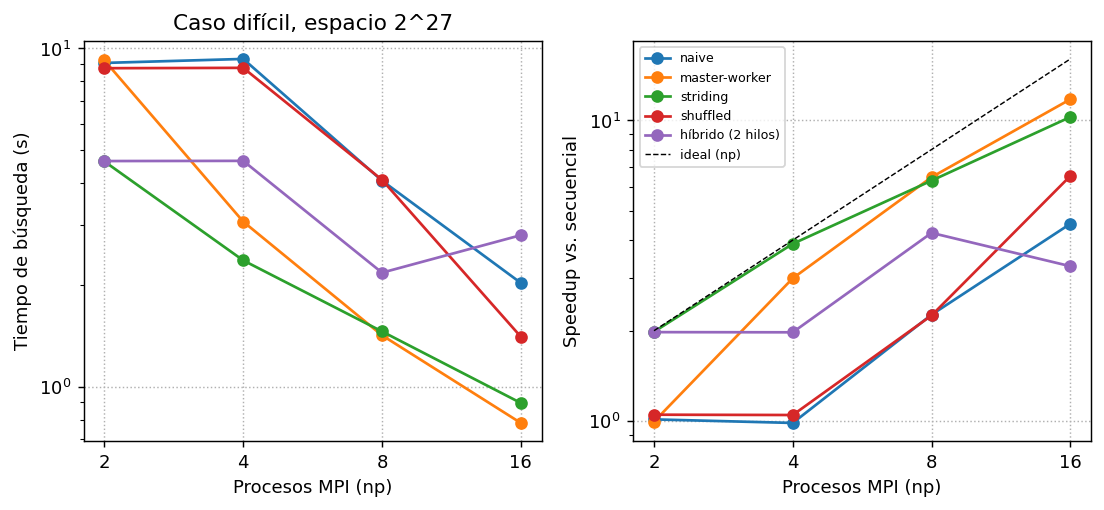
\includegraphics[width=\textwidth]{../results/np_scaling.png}
\caption{Tiempo y speedup con el número de procesos (caso difícil, $N=2^{27}$).}
\label{fig:np}
\end{figure}

Naive no mejora entre $np=2$ y $np=4$ (la llave sigue en el bloque del
proceso~0) y baja a saltos al achicarse los bloques ($np=8,16$). Striding
escala casi linealmente (speedups 1.98, 3.89, 6.31, 10.3; eficiencia 0.64 en
$np=16$, probablemente por los núcleos E y SMT de la CPU, como en la Sección~\ref{sec:hilos}). Master-worker rinde $\approx np-1$ (con
$np=2$ hay un solo trabajador). Shuffled sigue el patrón por bloques de
naive con esta llave. El híbrido (hilos libres, \texttt{--bind-to none}) hace en cada bloque la mitad
del tiempo de naive (4.65 vs. 9.06--9.31\,s con $np=2,4$ y 2.18 vs. 4.07\,s con $np=8$). Con $np=16$ son 32 hilos
sobre 20 núcleos lógicos y empeora (2.81\,s). La Figura~\ref{fig:np} resume el escalado.

El código completo está en \url{https://github.com/angelesquit/pry2-cpd}. Pasos para reproducir las pruebas.

\begin{lstlisting}[language=bash]
export PATH="/usr/lib64/openmpi/bin:$PATH"   # si mpirun no esta en PATH
make
chmod +x scripts/benchmark.sh
./scripts/benchmark.sh 4 180 2  # np=4, timeout=3 min, 2 hilos OpenMP
python3 scripts/speedup.py      # genera tabla + graficas en results/
./scripts/random_keys.sh 30 4 2 # 30 llaves aleatorias, N=2^24 (~7 min)
python3 scripts/random_summary.py   # tabla y grafica de variabilidad
\end{lstlisting}

\subsection*{Extras}

\begin{itemize}[nosep]
    \item \textbf{Cluster MPI en 2+ máquinas.} no intentado.
    \item \textbf{OpenMP + MPI.} \texttt{hybrid\_mpi\_omp.c}. Con 2 hilos tarda la mitad que naive con el mismo \texttt{np} en los casos media y difícil, y más lento en el fácil (Tabla~\ref{tab:comparativa}).
    \item \textbf{3+ acercamientos adicionales.} master-worker, striding, shuffled e híbrido, todos medidos en la Tabla~\ref{tab:comparativa}.
\end{itemize}

% =======================================================================
\section{Bibliografía}
% =======================================================================

\begin{enumerate}
    \item Stallings, W. (2017). \textit{Cryptography and Network
    Security: Principles and Practice} (7.ª ed.). Pearson. Capítulo 3,
    Block Ciphers and the Data Encryption Standard.

    \item National Institute of Standards and Technology (NIST).
    (1999). \textit{Data Encryption Standard (DES)} (FIPS PUB 46-3).
    U.S. Department of Commerce.
    \url{https://csrc.nist.gov/publications/detail/fips/46/3/final}

    \item Gropp, W., Lusk, E., \& Skjellum, A. (2014). \textit{Using
    MPI: Portable Parallel Programming with the Message-Passing
    Interface} (3.ª ed.). MIT Press.

    \item OpenSSL Project. (2024). \textit{DES routines --- OpenSSL 3.x
    documentation}.
    \url{https://www.openssl.org/docs/man3.0/man3/DES_ecb_encrypt.html}

    \item OpenMP Architecture Review Board. (2021). \textit{OpenMP
    Application Programming Interface} (versión 5.2).
    \url{https://www.openmp.org/specifications/}
\end{enumerate}

\end{document}
